\documentclass[tikz,border=8pt]{standalone}
\usepackage{amsmath,amssymb}
\usetikzlibrary{arrows.meta,automata,positioning,quotes}
\begin{document}
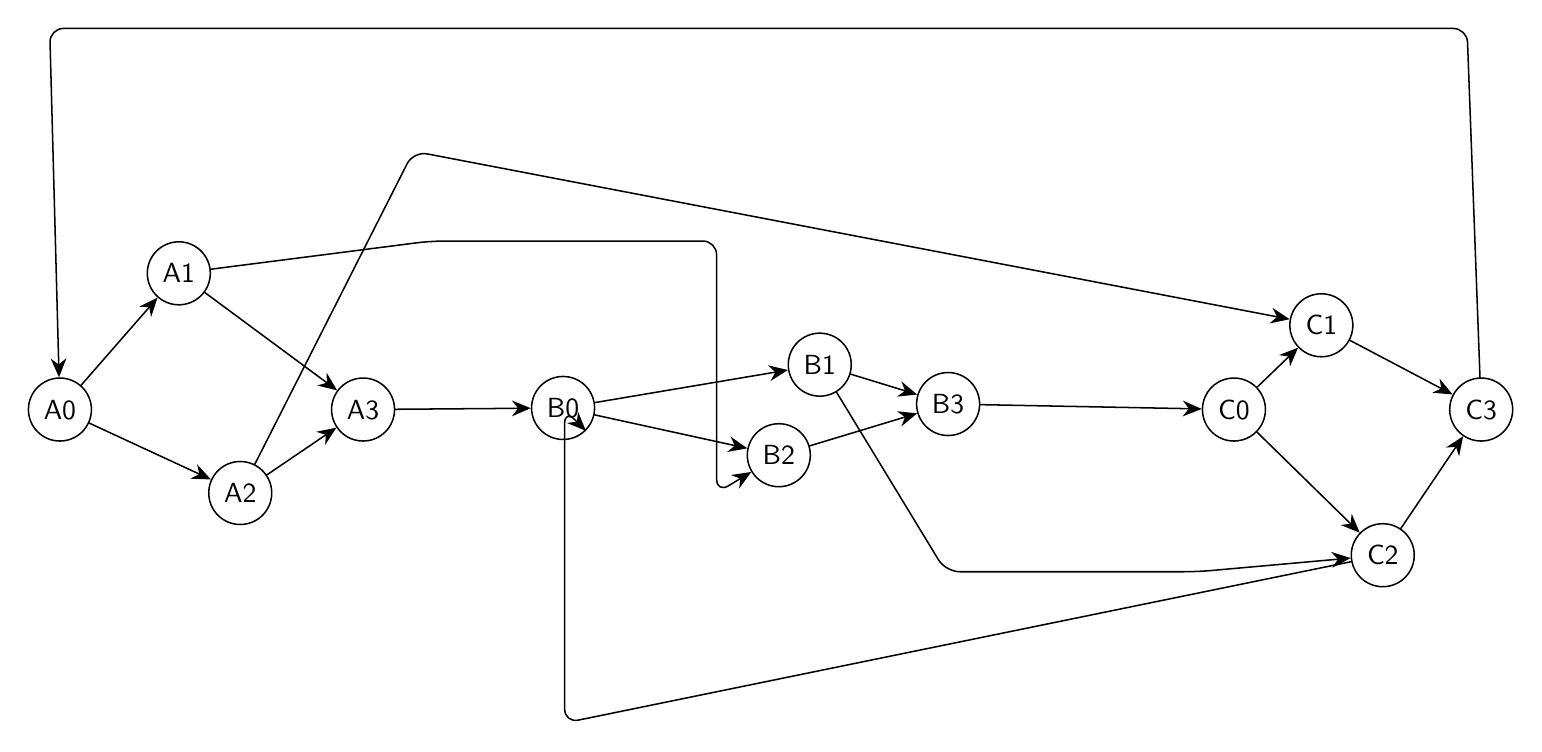
\begin{tikzpicture}[x=1cm,y=1cm]
\tikzset{
  graphnode/.style={circle,draw=black,line width=0.55pt,minimum size=8mm,inner sep=1pt,font=\sffamily},
  graphedge/.style={draw=black,line width=0.55pt,line cap=round,line join=round},
  directed/.style={graphedge,-{Stealth[length=2.4mm,width=2.0mm]}},
  undirected/.style={graphedge}
}
\node[graphnode] (n_A0) at (-8.87,-0.43) {A0};
\node[graphnode] (n_A1) at (-7.36,1.30) {A1};
\node[graphnode] (n_A2) at (-6.58,-1.49) {A2};
\node[graphnode] (n_A3) at (-5.02,-0.43) {A3};
\node[graphnode] (n_B0) at (-2.48,-0.41) {B0};
\node[graphnode] (n_B1) at (0.78,0.14) {B1};
\node[graphnode] (n_B2) at (0.26,-1.01) {B2};
\node[graphnode] (n_B3) at (2.41,-0.36) {B3};
\node[graphnode] (n_C0) at (6.04,-0.43) {C0};
\node[graphnode] (n_C1) at (7.15,0.64) {C1};
\node[graphnode] (n_C2) at (7.93,-2.28) {C2};
\node[graphnode] (n_C3) at (9.18,-0.43) {C3};
\draw[directed] (n_A0) -- (n_A1);
\draw[directed] (n_A0) -- (n_A2);
\draw[directed] (n_A1) -- (n_A3);
\draw[directed] (n_A2) -- (n_A3);
\draw[directed] (n_B0) -- (n_B1);
\draw[directed] (n_B0) -- (n_B2);
\draw[directed] (n_B1) -- (n_B3);
\draw[directed] (n_B2) -- (n_B3);
\draw[directed] (n_C0) -- (n_C1);
\draw[directed] (n_C0) -- (n_C2);
\draw[directed] (n_C1) -- (n_C3);
\draw[directed] (n_C2) -- (n_C3);
\draw[directed] (n_A3) -- (n_B0);
\draw[directed] (n_B3) -- (n_C0);
\draw[directed,rounded corners=5pt] (n_A1) -- (-4.16,1.71) -- (-0.53,1.71) -- (-0.53,-1.49) -- (n_B2);
\draw[directed,rounded corners=5pt] (n_A2) -- (-4.38,2.85) -- (n_C1);
\draw[directed,rounded corners=5pt] (n_B1) -- (2.38,-2.49) -- (5.58,-2.49) -- (n_C2);
\draw[directed,rounded corners=5pt] (n_C3) -- (9.00,4.41) -- (-9.00,4.41) -- (n_A0);
\draw[directed,rounded corners=5pt] (n_C2) -- (-2.46,-4.41) -- (-2.46,-0.43) -- (n_B0);
\end{tikzpicture}
\end{document}
